%  scripts/pkl_to_latex.py
% source PKL : thermal_v1_L8_Ne8_U10_t1_mode-uniform_tpall_t2all_tperpall_nmin2_solver-gcg_full_restarts8_iter200_kmax4_tol1em09_cut10_adaptive1_step5_clusteravg1_T0to0.5_N20-3c87501b406b_knone_diag0.pkl
% C_GME for n = 5-8 from the tail rerun (*_tailrerun.pkl, hpc_tail/merge_thermal_tail.py)
% scan type  : Tscan
% state      : gs
% x-max cap  : 0.3 (cut at k_B T/t = 0.3, supervisor 4 Nov 2026)
% requires   : \usepackage{pgfplots} \pgfplotsset{compat=1.18}
% colours match the matplotlib PDF (tab10 cycle)
\definecolor{gmeC0}{HTML}{1F77B4}
\definecolor{gmeC1}{HTML}{FF7F0E}
\definecolor{gmeC2}{HTML}{2CA02C}
\definecolor{gmeC3}{HTML}{D62728}
\definecolor{gmeC4}{HTML}{9467BD}
\definecolor{gmeC5}{HTML}{8C564B}
\definecolor{gmeC6}{HTML}{E377C2}
\definecolor{gmeC7}{HTML}{17BECF}

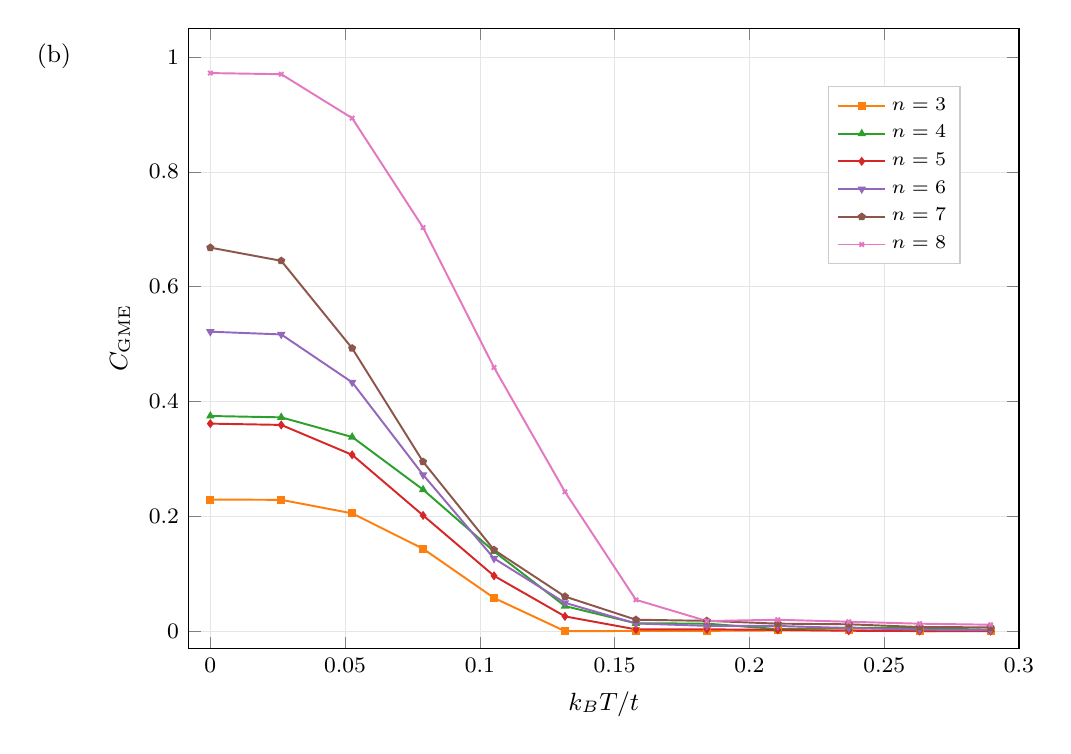
\begin{tikzpicture}
  \begin{axis}[
    width=\columnwidth,
    height=0.78\columnwidth,
    xlabel={$k_B T/t$},
    ylabel={$C_{\mathrm{GME}}$},
    grid=both,
    grid style={line width=.1pt, draw=gray!20},
    tick label style={font=\footnotesize\rmfamily, /pgf/number format/fixed},
    label style={font=\small\rmfamily},
    scaled ticks=false,
    legend style={font=\scriptsize\rmfamily, draw=gray!40, at={(0.5,1.03)}, anchor=south, /tikz/every even column/.append style={column sep=6pt}},
    legend cell align={left},
    legend columns=1,
    ymin=-0.03,
    ymax=1.05,
    xmin=-0.008,
    xmax=0.3,
    xtick={0,0.05,0.1,0.15,0.2,0.25,0.3},
    legend style={at={(0.850,0.763)}, anchor=center, fill=white},
    after end axis/.append code={\node[anchor=east, font=\small\rmfamily] at (axis description cs:-0.13,0.954) {(b)};},
  ]
    \addplot[color=gmeC1, mark=square*, mark size=1.1pt, line width=0.7pt] coordinates {
        (0,0.229253) (0.026316,0.228691) (0.052632,0.205165) (0.078947,0.143526)
        (0.105263,0.057789) (0.131579,0.000037) (0.157895,0.000338) (0.184211,0.000548)
        (0.210526,0.001244) (0.236842,0.001602) (0.263158,0.000044) (0.289474,0.00089)
    };
    \addlegendentry{$n=3$}
    \addplot[color=gmeC2, mark=triangle*, mark size=1.1pt, line width=0.7pt] coordinates {
        (0,0.3747) (0.026316,0.37237) (0.052632,0.338121) (0.078947,0.24646)
        (0.105263,0.138824) (0.131579,0.043655) (0.157895,0.013756) (0.184211,0.013166)
        (0.210526,0.00353) (0.236842,0.006102) (0.263158,0.005214) (0.289474,0.002593)
    };
    \addlegendentry{$n=4$}
    \addplot[color=gmeC3, mark=diamond*, mark size=1.1pt, line width=0.7pt] coordinates {
        (0,0.361429) (0.026316,0.35918) (0.052632,0.307082) (0.078947,0.201596)
        (0.105263,0.096367) (0.131579,0.02572) (0.157895,0.003121) (0.184211,0.003221)
        (0.210526,0.00226) (0.236842,0.000736) (0.263158,0.00023) (0.289474,0.000141)
    };
    \addlegendentry{$n=5$}
    \addplot[color=gmeC4, mark=triangle*, mark size=1.1pt, mark options={rotate=180}, line width=0.7pt] coordinates {
        (0,0.521524) (0.026316,0.516758) (0.052632,0.433346) (0.078947,0.272261)
        (0.105263,0.126641) (0.131579,0.049413) (0.157895,0.01344) (0.184211,0.009238)
        (0.210526,0.009053) (0.236842,0.005497) (0.263158,0.002653) (0.289474,0.001667)
    };
    \addlegendentry{$n=6$}
    \addplot[color=gmeC5, mark=pentagon*, mark size=1.1pt, line width=0.7pt] coordinates {
        (0,0.667932) (0.026316,0.644975) (0.052632,0.492598) (0.078947,0.294986)
        (0.105263,0.141515) (0.131579,0.060307) (0.157895,0.019949) (0.184211,0.017965)
        (0.210526,0.013093) (0.236842,0.011988) (0.263158,0.007222) (0.289474,0.006668)
    };
    \addlegendentry{$n=7$}
    \addplot[color=gmeC6, mark=x, mark size=1.1pt, line width=0.7pt] coordinates {
        (0,0.97189) (0.026316,0.969891) (0.052632,0.893417) (0.078947,0.702852)
        (0.105263,0.459098) (0.131579,0.242702) (0.157895,0.054648) (0.184211,0.017664)
        (0.210526,0.01989) (0.236842,0.016446) (0.263158,0.013026) (0.289474,0.01124)
    };
    \addlegendentry{$n=8$}
  \end{axis}
\end{tikzpicture}
